\documentclass[10pt,a4paper,french,titlepage]{article}
\author{par Gabriel Caux et Léo Peyronnet : Binome numéro 3}
\title{La réussite des alliances}
\date{Février-Avril 2022}
\usepackage[utf8]{inputenc}
\usepackage[T1]{fontenc}
\usepackage{babel}
\usepackage{amsfonts}
\usepackage{amsthm}
\usepackage{mathtools}
\usepackage{lineno}
\usepackage{todonotes}
\usepackage{listings}
\usepackage[pdftex]{hyperref}
\usepackage{amssymb}
\usepackage{tabto}
\usepackage{pst-node}
\usepackage{listings}
\usepackage[linguistics]{forest}
\theoremstyle{definition}
\newtheorem{exmp}{Exemple} 
\usepackage{tikz-qtree}
\usepackage{tikz-qtree-compat}
\usepackage{linguex}
\usepackage{geometry}
\geometry{hmargin=3cm,vmargin=1.5cm}


\lstset{
  aboveskip=3mm,
  belowskip=-2mm,
  basicstyle=\footnotesize,
  breakatwhitespace=false,
  breaklines=true,
  captionpos=b,
  commentstyle=\color{red},
  deletekeywords={...},
  escapeinside={\%*}{*)},
  extendedchars=true,
  framexleftmargin=16pt,
  framextopmargin=3pt,
  framexbottommargin=6pt,
  frame=tb,
  keepspaces=true,
  keywordstyle=\color{blue},
  language=C,
  literate=
  {²}{{\textsuperscript{2}}}1
  {⁴}{{\textsuperscript{4}}}1
  {⁶}{{\textsuperscript{6}}}1
  {⁸}{{\textsuperscript{8}}}1
  {€}{{\euro{}}}1
  {é}{{\'e}}1
  {è}{{\`{e}}}1
  {ê}{{\^{e}}}1
  {ë}{{\¨{e}}}1
  {É}{{\'{E}}}1
  {Ê}{{\^{E}}}1
  {û}{{\^{u}}}1
  {ù}{{\`{u}}}1
  {â}{{\^{a}}}1
  {à}{{\`{a}}}1
  {á}{{\'{a}}}1
  {ã}{{\~{a}}}1
  {Á}{{\'{A}}}1
  {Â}{{\^{A}}}1
  {Ã}{{\~{A}}}1
  {ç}{{\c{c}}}1
  {Ç}{{\c{C}}}1
  {õ}{{\~{o}}}1
  {ó}{{\'{o}}}1
  {ô}{{\^{o}}}1
  {Õ}{{\~{O}}}1
  {Ó}{{\'{O}}}1
  {Ô}{{\^{O}}}1
  {î}{{\^{i}}}1
  {Î}{{\^{I}}}1
  {í}{{\'{i}}}1
  {Í}{{\~{Í}}}1,
  morekeywords={*,...},
  numbers=left,
  numbersep=10pt,
  numberstyle=\tiny\color{black},
  rulecolor=\color{black},
  showspaces=false,
  showstringspaces=false,
  showtabs=false,
  stepnumber=1,
  stringstyle=\color{gray},
  tabsize=4,
  title=\lstname,
}


\begin{document}
\maketitle
\tableofcontents
\section{La réussite des alliances: structuration du jeu}
\subsection{Rappel des règles du jeu}
Quelques rappels des règles: \\
Prenez un paquet de cartes (32 ou 52) mélangez le pour créer une pioche, ensuite tirez les cartes une par une en les posant de gauche à droite faces visibles. Une fois que trois cartes ont été posées vous pouvez commencer à jouer. On procédera ainsi, on suppose que la carte la plus à gauche est la numéro une la carte à sa droite la numéro deux celle à sa droite numéro trois et ainsi de suite. Si la carte numéro trois a une similarité (même couleur ou même valeur) avec la carte numéro une il y a alors alliance de cartes, vous pouvez alors faire un saut dans ce cas-là la carte qui est située entre nos deux cartes passe sur le tas de celle qui la précède. Si aucun saut n'est possible il faudra continuer à piocher les cartes jusqu'à ce qu'un ou plusieurs saut soit possible le jeu s'arrête lorsqu'il n'est plus possible de piocher une carte et qu'il n'est pas possible de faire de saut non plus. On compte alors le nombre de tas restant et selon le nombre de tas requis pour gagner vous savez si oui ou non vous avez réussi.

\subsection{Création des fonctions (partie guidée)}
Pour représenter informatiquement le jeu de la réussite des alliances, nous avions à notre disposition une partie guidée intégrée au sujet. Ce "cahier des charges" détaillé nous a fourni un certain confort quant à l'architecture du programme en lui-même. En effet, comme les entrées, sorties et effets de bords de nos fonctions nous étaient déjà indiqué, nous n'avions pas à réfléchir à comment nos fonctions allaient interagir entre elles. Les appels à des fonctions antérieures, s'il y en avait, nous étaient eux aussi indiqués ou tout du moins suggérés. Cette souplesse de travail nous a permis de nous concentrer sur l'algorithmique de nos fonctions et comment optimiser ces dernières.\\

Néanmoins, le sujet nous permettait également de prendre certaines libertés. Par exemple, il nous était suggéré de réaliser des fonctions auxiliaires pour programmer la fonction "$une\_etape\_reussite$". C'est ce que nous avons fait avec la fonction "$piocher$" qui compartimente l'action de piocher une carte. Elle prend en argument deux listes, une qui représente la liste des tas de la réussite, l'autre qui représente la pioche. Elle a pour effet de bord de déplacer la première carte de la pioche (c'est à dire d'indice 0) au dernier emplacement de la liste des tas. Pour cela, nous avons utilisé la fonction "$pop$" qui a elle-même pour effet de bord de supprimer un élément d'une liste à un index précis et qui retourne cet élément. Nous avons donc redirigé la sortie de la fonction "$pop$" comme ceci : \\

\begin{lstlisting}
	def piocher(liste_tas,pioche):
    		liste_tas+=[pioche.pop(0)]

\end{lstlisting}

~~~fonction : ligne 118\\



Nous n'avons cependant pas jugé nécessaire de faire d'autres compartimentations pour fluidifier cette fonction.\\

La fonction "$reussite\_mode\_manuel$" nous a permis à nouveau de pouvoir prendre des libertés cette fois-ci quant à l'affichage des éléments et plus globalement l'interface utilisateur. Pour rappel, cette fonction a pour but de laisser l'utilisateur jouer une partie. Ceci nécessite une interface pour que l'utilisateur puisse choisir ce qu'il veut faire. Ainsi, afin de présenter au mieux ses options de jeu à l'utilisateur, nous avons réalisé un menu contenant un choix pour piocher, un choix pour réaliser un saut et un choix pour mettre fin à la partie. En plus de ce menu, nous avons décidé de réaliser un affichage de la réussite plus poussé permettant de relier chaque carte à un nombre et ainsi faciliter la sélection de la carte à faire sauter. 
Pour cela, nous avons réalisé la fonction "$afficher\_reussite\_num$". Elle prend pour argument la liste de cartes à afficher, ne revoie rien et a pour effet de bord l'affichage détaillé de la réussite. Cette fonction consiste en 3 boucles affichant respectivement les cartes de la réussite, les
accents circonflexes permettant de souligner les cartes, et les nombres désignant les cartes. A noter que bien que semblant être des index, ces nombres n'en sont pas tout à fait car : soit une liste $li$, $u$ l'index d'un élément de cette liste et $v$ un des nombres utilisés dans la fonction , alors:

\begin{align*}
	&u \in [0;(len(li)-1)] \iff [0;len(li)[\\
	&v \in [1;len(li)]
\end{align*}

Lors de la création de cette fonction, nous avons constaté des bugs survenant lors de l'affichage de grandes listes de cartes comme une pioche entière d'un jeu de 52 cartes. A raison de 4 caractères imprimés par carte (les 3 caractères de la carte $+$ l'espace de fin du print), l'affichage entier d'un jeu de 52 cartes correspond à l'impression de $4\times52=208$ caractères. Cela peut être un problème si l'utilisateur possède un petit écran et par conséquent un petit terminal. Les trois lignes de 208 caractères peuvent "déborder" chacune leur tour, provoquant des bugs similaires à celui-ci: \\\\
\begin{center}
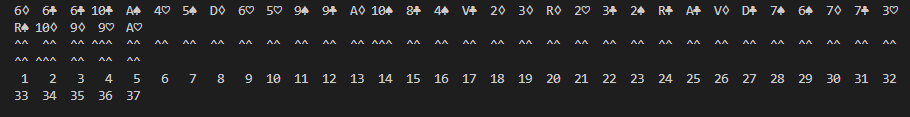
\includegraphics[scale=0.5]{img/bug_afficher_reussite_num.PNG}
\end{center}

Nous avons résolu ce problème en imbriquant les trois boucles d'affichage dans une plus grande boucle, et en changeant la condition de la première boucle. Maintenant, la première boucle conditionne les deux suivantes puisqu'elles sont des boucles "$for$" tournant sur une liste ($li\_dix$) ayant un nombre d'éléments équivalent au nombre de passage dans la première boucle. Cette boucle s'arrête soit lorsqu'il n'y a plus de cartes dans la liste, soit si l'affichage dépasse la taille du terminal. 

Le compteur "$y$" est incrémenté à chaque passage dans la boucle, c'est à dire à chaque impression de carte. Il permet donc de savoir où nous en sommes dans la lecture/impression de la réussite et par conséquent, poser une condition de sortie de boucle lorsque qu'on arrive au bout de la liste de cartes. Le compteur "$i$" qui est incrémenté lui aussi à chaque impression mais réinitialisé à chaque passage dans la grande boucle (ce qui reviens à une réinitialisation à la sortie de la "petite" boucle). 

Donc, multiplié par 4, il permet de compter le nombre de caractères imprimés à chaque passage de grande boucle. Il faut maintenant connaître la largeur du terminal pour pouvoir la comparer à "$i$". Pour obtenir la taille du terminal, nous avons utilisé le module intégré à python : "$shutil$". Avec la fonction "$get\_terminal\_size$", on peut obtenir le nombre de caractères que peut contenir le terminal en longueur. Ainsi, nous pouvons construire la deuxième condition de sortie de boucle en spécifiant que la boucle est valide tant que $i \times 4$ est inférieur ou égal à la largeur du terminal. Après modifications, la fonction est donc comme suit :

\begin{lstlisting}
def afficher_reussite_num(liCartes):
    columns, rows = shutil.get_terminal_size()
    i=0
    y=0
    li_dix=[]
    cpt=1
    while y<len(liCartes):
        i=1
        li_dix=[]
        while i*4<=columns and y<len(liCartes): 
            carte=liCartes[y]
            print(carte_to_chaine(carte),end=" ")
            if carte["valeur"]==10:
                li_dix+=[True]
            else:
                li_dix+=[False]
            y+=1
            i+=1
        print()
        for dix in li_dix:
            if dix:
                print("^"*3,sep="",end=" ")
            else:
                print(" ","^"*2,sep="",end=" ")
        print()
        for dix in li_dix:
            if cpt<10:
                print(" "*2,cpt,sep="",end=" ")
            else:
                print(" ",cpt,sep="",end=" ")
            cpt+=1
        print("\n")
\end{lstlisting}
~~~fonction: ligne 24



\section{Les Extensions: ajouts de fonctionnalités.}
\subsection{Vérification de la pioche}
Parmi les idées d'extensions que propose le sujet, nous avons choisi la fonction permettant de vérifier que la pioche de cartes ne soit pas truquée. Nommée "$vérifier\_pioche$", elle prend en arguments la liste que l'on souhaite vérifier ainsi que le nombre de cartes qu'elle contient - ou tout du moins qu'elle est censée contenir ! Elle n'a pas d'effets de bord et renvoie un booléen pour statuer de la conformité de la pioche : True si la pioche est conforme et False si la pioche est truquée. Notre algorithme se base sur la comparaison de la liste passée en argument avec une liste conforme. Une pioche peut être truquée de différentes manières :
\begin{itemize}
\item on peut ajouter les cartes que l'on souhaite directement dans la liste, auquel cas la taille de la liste doit être trop grande.
\item on peut sinon placer les cartes que l'on souhaite à l'index d'une autre carte. On remplace donc une carte par une autre, ce qui reviens à réécrire les cartes pour qu'elles nous arrangent. Il faudra donc veiller à ce qu'il n'y est pas de double. Pour cela, et comme nous savons que la taille de la liste sera contrôlée ensuite, il nous suffit juste de veiller à ce que toutes les cartes présentes dans une pioche conventionnelle le soient aussi dans la pioche que l'on contrôle. Ainsi, s'il y a des doubles, cette dernière sera forcément d'une taille non conforme.
\end{itemize}

Nous avons donc fait appel à notre fonction "$init\_pioche\_alea$" crée lors de la partie guidée qui permet de générer une pioche de 32 ou 52 cartes mélangées aléatoirement\label{piochealea}. Cette pioche nous sert donc de comparaison. Nous passons tout d'abord en revue la pioche suspecte en veillant à ce que chaque carte de la pioche conforme soit dans la pioche suspecte. Si ce n'est pas le cas, la fonction renvoie False. La fonction procède ensuite à une vérification de la longueur de la pioche suspecte. Pareil, si la pioche a plus de cartes qu'elle ne devrait en avoir, la fonction renvoie False. Si la pioche possède toutes les cartes de la pioche conforme tout en ayant le bon nombre de cartes, alors la fonction renvoie True.

\subsection{Statistiques}
Nous avons aussi choisi deux fonctions liées aux statistiques : \\
La première étant nommée "$res\_multi\_simulation$" qui va comme son nom l'indique nous servir à faire de multiples simulations de parties en même temps. Elle prend en argument le nombre de simulation que nous voulons faire ainsi que le nombre de carte que notre jeu contient. Voilà comment cette fonction procède, elle crée d'abord une boucle qui va faire appel à deux fonctions de la partie guidée, "$init\_pioche\_alea$" qui comme décrite précédemment génère une pioche de 32 ou 52 cartes mélangées aléatoirement ainsi que "$reussite\_mode\_auto$" qui permet de jouer une partie de réussite des alliances automatiquement. Ces deux fonctions nous permettent de faire des simulations différentes à chaque boucle. Après avoir fait chaque simulation de partie elle rajoute le résultat dans une liste qui est finalement renvoyée à la fin de la fonction. Cette liste qui est renvoyée correspond donc aux nombres de tas restants pour chaque simulation.\\

La seconde fonction se nomme "$statistiques\_nb\_tas$" elle va nous servir à connaitre certaines statistiques. Elle prend en argument le nombre de simulation que nous souhaitons faire ainsi que le nombre de carte contenu dans le jeu (32 ou 52). Cette fonction a pour but de faire un nombre défini de simulation puis de trouver ou calculer la moyenne, le maximum ainsi que le minimum de tas obtenus. Pour faire cela elle va d'abord faire appel à la fonction "$res\_multi\_simulation$" vu précédemment qui va servir à donner une liste depuis laquelle nous allons pouvoir calculer les statistiques dont nous avons besoins pour cela nous allons créer une boucle qui va nous servir à trois choses : premièrement grâce à cette boucle nous allons pouvoir additionner toutes les valeurs d'une liste dans une seul variable. Nous allons aussi pouvoir trouver le maximum et le minimum en comparant les valeurs entre elles.

Une fois sorti de cette boucle nous pouvons alors diviser notre variable moyenne par la longueur de la liste pour trouver la moyenne. Cette fonction nous affiche donc la moyenne, le maximum et le minimum de tas pour un nombre prédéfinis de simulations. Grâce à cette fonction nous avons pu voir que pour dix milles simulations il y a 21.133 tas en moyenne 2 au minimum et 47 au maximum.


\subsection{Probabilités}
Pour finaliser nos extensions, nous avons décidé de compléter notre partie "$Statistiques$" avec une partie "$Probabilités$". Nous avons réalisé dans un premier temps la fonction "$proba$" qui nous permet de calculer les pourcentages de réussite en fonction du nombre de tas de cartes maximum pour gagner. Cette fonction ne prend comme argument optionnel que le nombre de cartes présentes dans le jeu (32 ou 52), n'a pas d'effets de bord et retourne une liste contenant les pourcentages de réussite triés par ordre croissant du nombre palier de réussite. L'appel à la fonction précédemment présentée "$res\_multi\_simulation$" constitue la base de notre algorithme. Pour rappel, elle permet d'obtenir une liste d'entiers correspondants aux nombres de tas restant respectivement à la fin de chaque réussite simulée.
Donc, si nous réalisons cent simulations, nous pouvons compter combien respectent le palier de réussite et donc établir un pourcentage de victoire avec tel palier de réussite.\\

Ainsi, une boucle "for" se charge de vérifier si chaque valeur de la liste est inférieure ou égale au nombre palier. Si oui, une variable "$prctage$" 
correspondante au pourcentage est incrémentée. Au bout des cent passages de boucle, la valeur de cette variable est ajoutée à la liste de retour puis est remise à zéro. Cette remise à zéro permet l'itération des étapes décrites dans une grande boucle "$while$" ayant pour condition de sortie qu'un compteur soit supérieur au nombre de cartes du jeu. Ce compteur se nomme "i" et représente le nombre palier pour la réussite. Ainsi, en l'incrémentant à la fin de chaque passage dans sa boucle on peut établir le pourcentage de réussite pour les différentes valeurs de palier. Nous pouvons représenter notre fonction comme suit : 
Soit $i$ le compteur du même nom, $y$ le compteur permettant de parcourir la liste retourné par "$res\_multi\_simulation$"\footnote{y n'est pas présent dans le code mais est algorithmiquement sous-entendu par la boucle "$for$".}, $li$ la liste que retourne "proba", et $c$ le nombre de cartes du jeu \footnote{c est représenté par l'argument optionnel "$nb\_cartes$" dans le code de "$proba$".} (32 ou 52), alors:

\begin{center}
\begin{tabular}{|p{3cm}|l|c|r|}
  \hline
  nombre de palier pour victoire & 2 & i & c\\
  \hline
  valeur de la liste & li[0] & li[y] & li[$c-2$] \\
  \hline
\end{tabular}
\end{center}
Donc :
\begin{align*}
&i \in [2;c]\\
&y \in [0;c-2]
\end{align*}
Nous disposons maintenant de pourcentages décrivant les probabilités de réussite des alliances en fonction d'un certain nombre de tas restant à la fin 
de la partie. Nous avons créé une seconde fonction nommée "$affiche\_proba$" afin de représenter graphiquement les probabilités de victoire. Comme la fonction "$proba$",
"$affiche\_proba$" a pour seul argument un entier indiquant le nombre de cartes présentes dans le jeu. Cependant, elle ne renvoie rien et a pour effet de bord l'affichage
du graphique. Nous avons fait appel dans un premier temps à notre fonction "$proba$" afin de remplir notre axe des ordonnées. Les valeurs en abscisses sont générées par une boucle
"for". Nous pouvons exprimer x et y, respectivement pour les abscisses et les ordonnées comme ceci, avec c le nombre de cartes du jeu :
\begin{align*}
&x \in [2;c] \\
&y \in [0;100]
\end{align*}
Pour l'affichage, nous avons fait appel au module python "$matplotlib.pyplot$" donnant accès à de nombreuses fonctions d'affichage graphique. Pour notre part, nous avons
dans un premier temps utilisé la fonction "$plot$" permettant de créer le graphique en lui passant en argument les listes représentant les différents axes du graphique.
Pour rendre le graphique plus compréhensible, nous avons également utilisé les fonctions "$xlabel$" et "$ylabel$" permettant de donner un titre aux abscisses et aux
ordonnées. Pour finir, afin d'afficher le graphique, nous avons utilisé la fonction "$show$".



\section{Le debug$\_$mode}
\subsection{Introduction}
Nous sommes arrivés à un moment dans le projet ou nous avions du mal à tester nos fonctions et l’interface de notre main ne nous convenais pas. Nous avons alors décidé de créer un espace de test de fonction qui serait plus facile et plus rapide pour tester différentes fonctions avec différentes entrées. Il nous est alors venu à l’esprit de faire un debug$\_$mode qui nous permettrait de tester toutes nos fonctions facilement et rapidement.
\subsection{Structure du programme}
Notre débug$\_$mode se présente donc comme un répertoire de l'ensemble de nos fonctions. Il permet d'y faire appel via une interface prenant en charge le choix des arguments (listes, entiers, chaines de caractères). Il prends également en compte un gestion des fichiers de sauvegardes.  Les fonctions sont présentées dans un menu à choix multiples et rangées par rubriques. Par exemple, les fonctions d'affichage sont rangées dans le premier choix du menu: "1.Fonctions d'affichage". Un sous-menu s'affiche alors pour sélectionner la fonction dans sa rubrique. L'utilisateur peut à tout moment revenir au menu principal avec le choix "r.Retour" et quitter le programme avec le choix présent dans le menu principal "q.Fermer debug$\_$mode". Des variables sont également incluses dans le programme. Elles permettent de sauvegarder pendant la durée de l'utilisation du programme des cartes, des listes
de cartes, etc ... Nous avons implémenté dans notre programme:
\begin{align*}
&-4~listes~:~"liCartes", "liCartes2", "liCartes3~et~"liFichier"\\
&-2~dictionnaires~:~"carte1"~et~"carte2"\\
&-une~chaîne~de~caractères~:~"car"\\
&-un~entier~(négligeable)~:~"entier"\\
\end{align*}
Les listes servent de listes de cartes, c'est à dire de listes de dictionnaires, sauf liFichier dont la fonction sera détaillée ci-dessous. Les dictionnaires représentent des cartes conforme à celles que le sujet demande. \\
Ces variables peuvent être utilisées à la guise de l'utilisateur via les différentes fonctions. Le menu principal est accompagné d'un tableau affichant les valeurs des 
différentes variables. Pour éclaircir notre code, nous avons compartimenté l'affichage de ce tableau dans la fonction "$tabVar$". Elle ne prend par conséquent aucun
argument ni ne renvoie rien. Cette fonction fait d'abord appel à la fonction "$texte\_encadre$" qui permet d'entourer un texte avec des '=' pour le mettre en valeur. Nous affichons donc le titre du tableau puis les différentes variables avec leurs valeurs. Comme le tableau s'affiche en même temps que le menu, si une variable
viens à être modifié par une fonction, sa valeur mise à jour sera affiché dans le tableau à la fin de l'appel de la fonction.
Lorsqu'une fonction est sélectionnée dans le menu, les variables doivent être sélectionnées avant que l'appel à la fonction ne soit fait.\\ La fonction "$choixVar$" permet d'afficher à l'utilisateur les variables pour qu'il puisse en choisir une. Elle prend comme argument une chaine de caractère représentant le type de variable
que l'utilisateur doit choisir. Ainsi, si l'utilisateur veut réaliser un appel à la fonction "$carte\_to\_chaine$", prenant pour unique argument un dictionnaire, le programme principal de debug$\_$mode fera appel à sa fonction  " $choixVar$ " avec en argument la chaîne de caractère "c" (pour carte). Un menu s'ouvrira pour que l'utilisateur puisse choisir entre "carte1" et "carte2". Un appel à la fonction "$carte\_to\_chaîne$" sera ensuite réalisé dans le programme principal avec pour argument un des deux dictionnaires choisi.

\subsection{Gestion des fichiers}
Certaines fonctions peuvent cependant prendre comme argument des noms de fichiers, nous avons donc mis en place une gestion dynamique des fichiers présents dans le sous-répertoire "ressources" (voir structure du répertoire \ref{arbre}). La gestion des fichiers de notre programme s'articule autour de la fonction "$choixFichier$". Cette dernière permet à l'utilisateur de choisir un fichier existant présent dans le dossier "ressources", ou bien d'en créer un nouveau si c'est nécessaire. Elle ne prend pas d'argument et retourne le nom du fichier choisi ou crée. Afin que la gestion des fichiers soit dynamique et que par exemple, un fichier crée avec cette fonction puisse par la suite être sélectionné par cette même fonction, nous avons créé une liste "liFichier" qui répertorie l'ensemble des fichiers consultables. La fonction "$choixFichier$" consiste donc à lire ou modifier la liste "liFichier" ou fonction de ce que l'utilisateur choisi. Elle a donc comme effet de bord la modification de la variable "liFichier". Or cette variable est définie dans le programme principal, une fonction peut consulter mais pas modifier une variable issue du programme principal. Pour pallier ce problème, nous avons utilisé le mot-clé "global" qui permet de définir une variable comme globale, c’est-à-dire modifiable partout dans le programme. Plus précisément, nous avons déclaré "liFichier" comme étant globale mais dans la fonction "$choixFichier$". Cela revient donc à ce que "liFichier" soit globale uniquement pour la fonction "$choixFichier$", elle n'est ainsi pas réellement globale et ne peut pas être modifier par les autres fonctions comme la nomination "globale" le voudrait.
\begin{exmp}
Soit le programme suivant :
\begin{lstlisting}
def modif():
    global oui
    oui=5
def modifBis():
    oui=1
oui=1
modif()
modifBis()
print(oui)
\end{lstlisting}
Le programme affiche "5", la fonction "$modifBis$" ne modifie pas la variable "oui". Elle n'est donc globale que pour la fonction "$modif$".
\end{exmp}
\subsection{Limites et Erreurs}
\subsubsection{La redondance}
Lors du développement de debug$\_$mode, nous avons été confrontées à de multiples problèmes. Le premier, et selon nous plus important a été le manque de préparation et d'organisation dans la réalisation de la structure du programme. Nous n'avons pour ainsi dire pas réfléchis à l'architecture du programme, ou comment les différentes fonctionnalités de ce programme allaient exister entre elles. Alors que nous avions bien en tête l'objectif principal du programme, c’est-à-dire une interface utilisateur permettant de faciliter l'appel de fonctions pour les tester, nous n'avions pas encore réfléchi à comment réaliser cet objectif. Nous avons résolu ce problème au fur et à mesure du développement du programme. En résulte un programme manquant, à notre goût, d'une certaine rigueur dans l'exécution des tâches qu'il lui est demandé. La redondance dans les instructions est également selon nous un symptôme de cette mauvaise préparation. Par exemple, lorsqu’une fonction retourne une valeur, le programme principal répète la même instruction pour tous les choix de variables de l’utilisateur :
\begin{exmp}
\begin{lstlisting}
elif choix=="3":
	chVar=choixVar("lc")
    print("Création d'un jeu à 32 ou 52 cartes ?")
    chNbCartes=int(input("(ecrivez 32 pour le jeu à 32, n'importe 	quelle autre nombre pour le jeu à 52)"))
    if chVar=="lc1":
    		liCartes=fonctions.init_pioche_alea(chNbCartes)
    elif chVar=="lc2":
    		liCartes2=fonctions.init_pioche_alea(chNbCartes)
	elif chVar=="lc3":
		liCartes3=fonctions.init_pioche_alea(chNbCartes)
    else:
		print("Erreur: variable inconnue, code retour choixVar() 		inconnu")
    input("(Appuyer sur entrer pour revenir au menu)")
	conti=False
\end{lstlisting}
Le code de la ligne 228 à la ligne 237 représente une redondance car seul le nom de la variable recevant la valeur retour change.
\end{exmp}
Nous aurions pu pallier cette redondance en regroupant l'ensemble des variables pouvant être sélectionnées par l'utilisateur dans une liste ou un dictionnaire. Cela aurait nous aurait permis d'éviter la redondance de nos instructions car le choix de l'utilisateur aurait pu se porter sur l'indice d'une liste ou la clé d'une entrée de dictionnaire.
\begin{exmp}
Reprenons le dernier exemple.
\begin{lstlisting}

nomvar=[
    "carte1",
    "carte2",
    "liCartes",
    "liCartes2",
    "liCartes3",
    "car"
]
var=[
    {"valeur":"A","couleur":"C"},
    {"valeur":"R","couleur":"T"},
    [{"valeur":9,"couleur":"C"},{"valeur":10, "couleur":"K"},{"valeur":9,"couleur":"T"}],
    [],
    [],
    "random"
]

chVar=int(input("Quelle variable? (0,1,2,3,4 ou 5):"))
print("Création d'un jeu à 32 ou 52 cartes ?")
chNbCartes=int(input("(ecrivez 32 pour le jeu à 32, n'importe quelle autre nombre pour le jeu à 52)"))
var[chVar]=init_pioche_alea(chNbCartes)
input("(Appuyer sur entrer pour revenir au menu)")

print(var[chVar])
\end{lstlisting}
Nous avons ici utilisé une paire de liste, "nomvar" pour le nom des variables et "var" pour la valeur des variables. Comme vous pouvez le constater, nous n'avons plus besoin de nous répéter dans les instructions.
\end{exmp}
A noter que l'on aurait ainsi pu éviter l'utilisation des variables globales avec les fonctions de gestion de fichiers. Cette méthode meilleure en tout point à celle mise en place dans la version actuelle du programme aurait néanmoins nécessité une réécriture complète du code de debug$\_$mode pour être effective. Pour des raisons de gestion du temps, nous n'avons pas pu nous le permettre.
\subsubsection{Une gestion partielle des fichiers}
Un autre symptôme du manque d'architecture dans la réalisation d'un programme est l'ajout successif de fonctionnalités non prévues. Une gestion des fichiers s'est imposé lorsque nous avons essayé d'implémenter les fonctions \\"$init\_pioche\_fichier$" et "$ecrire\_fichier\_reussite$" dans notre interface utilisateur. Il devait pouvoir sélectionner le fichier désiré pour pouvoir le lire avec "$init\_pioche\_fichier$" mais également en créer de nouveaux pour pouvoir sauvegarder des listes de cartes avec "$ecrire\_fichier\_reussite$". Nous avons donc dans un premier temps créé "liFichier" permettant de pouvoir garder en mémoire le nom des fichiers créés par l'utilisateur. Cependant, cette mémoire était à court-terme car lorsque le programme était fermé, les modifications apportées à "liFichier" n'étaient pas sauvegardées. Nous avons donc dans un second temps créé un système de sauvegarde de la liste dans le fichier "liFich.csv". Malgré cet ajout, la gestion des fichiers reste partielle : l'utilisateur ne peut par exemple pas supprimer de fichiers via le debug$\_$mode. Ces défauts peuvent néanmoins se justifier par le fait que debug$\_$mode ne s'adresse pas à des utilisateurs "grand-public" mais plutôt à des utilisateurs connaissant et ayant accès au code de l'ensemble du projet (des développeurs).
\subsubsection{Une syntaxe conditionnelle lourde.}
Enfin, nous avons également pu relever que la syntaxe "if/elif/else" pouvait paraître elle aussi redondante, ou tout du moins lourde. Nous avons cherché des solutions en utilisant d'autres syntaxes conditionnelles comme "match-case". Semblable à la syntaxe "switch-case" en langage C, "match-case" nous aurait permis une syntaxe plus légère pour l'écriture de nos menus et sous-menus. Malheureusement, cette fonctionnalité est sortie avec le patch 3.10 de Python en octobre dernier. Jugeant cette date beaucoup trop proche et afin d'éviter d'éventuels conflits de versions de Python, nous avons renoncer à implémenter cette fonctionnalité.
\section{Interface utilisateur: proposer un produit fini.}
\section{Annexes}
\subsection{Structure du répertoire}\label{arbre}

Cette arbre montre la structure de notre répertoire.\\
\hspace*{\fill}
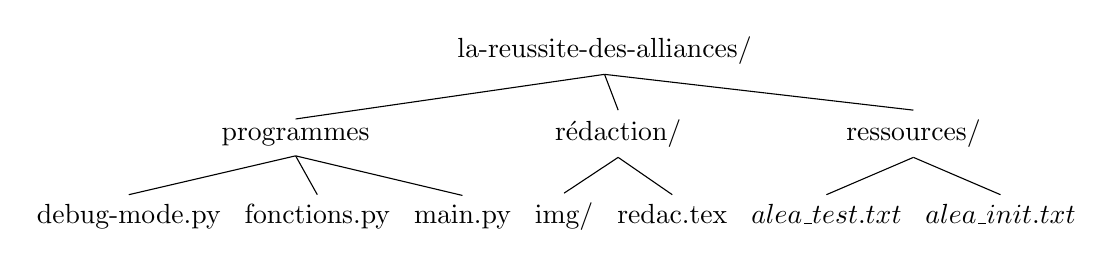
\begin{tikzpicture}[scale=1][baseline]
\Tree 
[.la-reussite-des-alliances/ 
	[.programmes debug-mode.py fonctions.py main.py 
    ] 
	[.rédaction/ img/ redac.tex 
    ] 
	[.ressources/ $alea\_test.txt$ $alea\_init.txt$
    ]
]
     \end{tikzpicture}%
     \hspace*{\fill}
\subsection{sources}
\begin{align*}
&-xm1math.net\\
&-https://stackoverflow.com/\\
&-overleaf.com\\
&-stackexchange.com
\end{align*}



Le liens de notre gitlab est :\url{https://gitlab.isima.fr/lepeyronne/la-reussite-des-alliances}
\end{document}
